\chapter{INTRODUCTION} \label{chap:introduction}
    %\doublespacing
    \minitoc
    
    %\newpage
    \begin{center}
    	\emph{Abstract of chapter \ref{chap:introduction}}
    \end{center}
    This chapter introduces the field of X-ray astronomy, highlighting its significance in studying high-energy celestial phenomena. It covers the advancements from early X-ray detectors to contemporary missions like Chandra and XMM-Newton, which have provided detailed spectral data of various X-ray sources. A special focus is on luminous supersoft X-ray sources (SSS), a distinct category identified by their exceptionally soft spectra and high luminosities. The chapter explores the prevailing models for SSS, primarily involving accreting white dwarfs in binary systems, and their potential as progenitors of Type Ia supernovae. It also delves into the classifications and companion star types within SSS systems, and the significance of understanding classical novae in the context of X-ray observations. Finally, it outlines the research problem, hypothesis, and objectives, aiming to develop robust models for SSS spectra and understand their underlying physical mechanisms.
    
    \section{Introduction} \label{introduction:introduction}
    	The pursuit of cosmic knowledge has been propelled by advancements in observational techniques across the electromagnetic spectrum.
 X-ray astronomy, in particular, offers a unique window into the high-energy universe, revealing phenomena inaccessible to other wavelengths. By probing celestial objects in the X-ray band, astronomers gain profound insights into extreme astrophysical environments dominated by processes such as accretion, stellar explosions, and the interplay of matter and radiation.
        
        \subsection{X-ray Astronomy} \label{introduction:introduction:x-ray-astro}
        	X-ray astronomy has emerged as a pivotal domain within the broader field of astronomy, providing invaluable insights into high-energy phenomena across the Milky Way and beyond. Observations made in the X-ray window enable us to understand many high-energy events in the Milky Way and other galaxies. By studying celestial objects in the X-ray spectrum, many significant strides have been made in unraveling the complexities of stellar and galactic evolution \cite{giacconi1962evidence}. Unlike visible light, however X-rays are entirely absorbed by Earth's atmosphere, necessitating observations from space-based platforms. Since the pioneering Uhuru mission in 1970, a succession of advanced X-ray telescopes has been deployed, leading to the discovery of a diverse array of exotic celestial X-ray sources, including black holes, neutron stars, white dwarfs and supernova remnants \cite{tanaka1996x}.
        	%Today X-ray astronomy is recognized as a mature and important branch of astronomy. Observations made in the X-ray window enable us to understand many high-energy events in the Milky Way and other galaxies. The physics of such events have improved our understanding of stellar and galactic evolution. Since our atmosphere is opaque to X-rays, observations in this band need to be carried out from outer space. Starting with the Uhuru in 1970, a series of satellites with X-ray telescopes have been launched, leading to the discovery of new and exotic classes of X-ray sources.
        	
        	%In X-ray astronomy, the principal mode of measurement is to detect individual photons so as to determine
        	X-ray astronomy relies on the detection and analysis of individual X-ray photons to extract critical information, namely its \emph{arrival direction}, \emph{energy}, \emph{time of arrival} and the \emph{polarization angle} \cite{overviewXrays}. Advancements in space-based X-ray observatory instrumentation have significantly enhanced spectral resolution, providing deeper insights into celestial X-ray sources. While early X-ray detectors primarily employed proportional and scintillation counters, the later development of Wolter-type focusing optics and imaging detectors marked a pivotal turning point, enabling the creation of two-dimensional X-ray images \cite{giacconi1962evidence}. Contemporary missions like Chandra and XMM-Newton utilize actively cooled, pixelated solid-state detectors as their focal plane instruments, offering superior energy resolution and broader energy coverage compared to their predecessors \cite{jansen2001xmm,weisskopf2000chandra}. Complementing imaging capabilities, these observatories also incorporate high-resolution grating spectrometers, providing exceptional spectral resolution and high throughput for detailed spectral analysis \cite{paragb2017rev}.
        	%The refinement of the instruments on board space-based X-ray observatories have led to greater spectral resolution of the observed X-ray objects.	Initially, X-ray detectors were proportional counters and scintillation counters. The introduction of focusing and imaging X-ray optics, the Wolter telescope, together with imaging detectors in the focal plane allowed the capture of 2D X-ray imagery. Today, the pioneering X-ray satellites, namely Chandra and XMM-Newton, have actively cooled pixelized solid-state detectors as their standard focal plane detector, providing higher energy resolution and wider energy range than proportional counters. In addition to imaging telescopes, high-resolution grating spectrometers, which have very high spectral resolution and large throughput, are also used in the Chandra and XMM-Newton missions \cite{paragb2017rev}.
        
        \subsection{Supersoft X-ray Sources} \label{introduction:introduction:sss}
        	Luminous supersoft X-ray sources (SSS) were initially identified as a distinct category of exceptionally bright X-ray emitters by Tr{\"u}mper \emph{et al.} \cite{trumper91}, Greiner \emph{et al.} \cite{greiner91}, and Kahabka \emph{et al.} \cite{kahabka06}. These objects are characterized by extraordinarily soft X-ray spectra peaking within the 15--80 eV energy range, corresponding to blackbody temperatures of approximately 300,000--500,000 K \cite{kahabka06}. Their immense X-ray luminosities, typically on the order of the Eddington limit ($\sim 10^{38}$ erg s$^{-1}$), place them among the most powerful X-ray sources known. The extreme softness of their spectra suggests a unique physical mechanism for their energy production, distinguishing SSS from other classes of luminous X-ray binaries.
        	%Luminous supersoft X-ray sources (SSS) were first identified as an important new class of intrinsically bright X-ray sources by Tr{\"u}mper \emph{et al.}\cite{trumper91}, Greiner \emph{et al.}\cite{greiner91} and Kahabka \emph{et al.}\cite{kahabka06}. SSS are now classified as sources with X-ray luminosities of the order of the Eddington limit ($\sim 10^{38}$ erg s$^{-1}$), and with extremely soft spectra peaking in the energy range 15--80 eV -- corresponding to a blackbody temperature of $\sim\,$300,000--500,000 K (Kababka \emph{et al.})\cite{kahabka97}.
        	
        	The initial discovery of luminous SSS can be attributed to the pioneering observations conducted by the Einstein and ROSAT satellites, which employed low-resolution proportional counters. These early detections laid the groundwork for subsequent, more detailed investigations. Notably, the Chandra and XMM-Newton observatories have provided high-resolution X-ray spectra for a substantial number of SSS, enabling unprecedented insights into their physical properties. Among the most extensively studied SSS are RX J0925.7-4758 \cite{bearda2002,motch2002}, CAL 83 \cite{lanz2005}, CAL 87 \cite{orio2004}, and RX J0019.8+2156 \cite{schwarz2004}, which have yielded particularly remarkable spectral data.
        	%The first SSS were observed by the low-resolution proportional counters on board the Einstein and ROSAT satellites. Presently, high-resolution X-ray spectra have been obtained by Chandra and XMM-Newton for a number of SSS, some of the most remarkable ones include RX J0925.7-4758 \cite{bearda2002,motch2002}, CAL 83 \cite{lanz2005}, CAL 87 \cite{orio2004} and RX J0019.8+2156 \cite{schwarz2004}.
        	
        	The prevailing model for luminous SSS posits that the majority of these objects are accreting white dwarfs (WDs) within binary systems. In these systems, hydrogen-rich material is transferred from a companion star onto the WD's surface, where it accumulates and undergoes thermonuclear burning \cite{vandenHeuvel92}. This sustained or intermittent hydrogen burning process is responsible for the observed intense, soft X-ray emission. While this model accounts for most SSS, its important to note that there are exceptions, such as isolated WDs undergoing final helium-shell flashes, which also exhibit supersoft X-ray characteristics.
        	%The currently accepted model for luminous SSS is that, with a few exceptions, these sources are accreting white dwarfs (WDs) within a binary system, \emph{which are burning hydrogen within their envelopes in a steady or intermittent manner} \cite{vandenHeuvel92}.
    
    \section{Background} \label{introduction:background}
    	Once considered enigmatic, the study of SSS has evolved into a cornerstone for understanding the evolution of X-ray binaries. A significant fraction of the identified SSS exhibit transient behaviour. These transient SSS are categorized into two primary groups: classical and symbiotic novae with a supersoft phase, and systems without documented nova outbursts but characterized by alternating ``on'' and ``off'' supersoft X-ray states. While the precise evolutionary pathway leading to Type Ia supernovae (SNe Ia) remains an active area of research, the calculated rates of these events align with the predicted outcomes of two leading progenitor scenarios: merging double degenerate white dwarfs and carbon-oxygen white dwarfs accreting from a non-degenerate companion (CBSS). The intricate spectra of many SSS, as captured by high-resolution grating spectrometers, prominently feature P Cygni profiles. Although accurate modelling of these spectra presents a formidable challenge but is essential for deriving fundamental parameters of the SSS under investigation.
        %From being a mere curio, today the study of SSS is regarded as being crucial to the understanding of the evolution of X-ray binaries. A large proportion of the SSS discovered so far are transient. Supersoft transients seem to be classical and symbiotic novae having a supersoft phase and also systems with no known nova outburst but exhibit supersoft X-ray ``on'' and ``off'' states. Although the evolution of type Ia supernovae (SN Ia) has not been fully solved as yet, keeping in mind their calculated numbers and birth rates, merging double degerate white dwarfs and CBSS are considered to be the two most promising progenitor candidates for SN Ia. The SSS spectra for several sources obtained with high-resolution grating spectrometers reveal the dominance of several spectral features, including P Cygni profiles. Obtaining a proper fit for such spectra has been challenging so far, but crucial in order to be able to derive the parameters of the SSS under study.
    
    \section{Current Status} \label{introduction:current_status}
		This section provides an overview of the current state of knowledge regarding observational data obtained from SSS.  It explores the key findings and challenges associated with analysing these data, drawing upon the latest research in the field.
        %A brief summary of the current literature concerning the study of observational data from SSS is discussed in the current section.
        
        \subsection{Supersoft X-ray Sources as a New Class of Luminous X-ray Sources} \label{introduction:current_status:new-class}
        	The initial discovery of luminous SSS was hindered by the limitations of the Einstein satellite, which possessed a restricted spectral range and resolution. Consequently, the first four SSS identified by this mission were initially classified alongside other, more typical high-luminosity X-ray sources, such as accreting neutron stars or black holes within binary systems \cite{long81,seward81}.
        	
        	It was the subsequent launch of the ROSAT satellite, equipped with enhanced spectral capabilities, that enabled SSS to be recognised as a distinct class of object. In contrast to the classical high-luminosity X-ray sources, SSS exhibited a characteristic spectral peak within the 15-80 eV energy band. This corresponds to blackbody temperatures approximately two orders of magnitude lower than those associated with accreting neutron stars or black holes \cite{kahabka97}.
        	%The limited spectral range and resolution of the Einstein satellite did not allow the first four luminous SSS discovered by it to be recognised as a separate class \cite{long81,seward81}. It was due to the enhanced spectral range and resolution of the ROSAT that SSS were later distinguished as a class of sources different from classical strong-point X-ray sources, such as accreting neutron stars or black holes in binaries. SSS have been observed to have a distinctive peak around 15--80 eV, corresponding to blackbody temperatures that are around 2 orders of magnitude lower than that of classical strong point X-ray sources.
        	
        \subsection{Currently Accepted Model for SSS} \label{introduction:current_status:SSS-model}
        	If the luminosity and effective temperature of a star are known, using the \emph{Stefan-Boltzmann's law}, one can derive its radius. The Stefan-Boltzmann's law is as follows
        	\begin{equation} \label{SSS-model:stef-boltz}
        		L=4\pi R^2\sigma T^4
        	\end{equation}
        	
        	Rearranging this equation yields:
        	\begin{equation} \label{SSS-model:star-radius}
        		R=9\times 10^8(L_{37.5})^{1/2}(T_e/40\,\mathrm{eV})^{-2}\,\mathrm{cm,}
        	\end{equation}
        	where $L_{37.5}$ is the X-ray luminosity in units of $10^{37.5}$ erg/s, and $T_e$ is the effective temperature in electron volts.
        	
        	Applying in equation (\ref{SSS-model:star-radius}) the characteristic values of SSS, i.e. $L_{37.5}=1$ and $T_e=40$, results in a radius of approximately 9000 km, closely resembling the size of a white dwarf. This similarity in radius, analogous to the relationship between accretion onto neutron stars or black holes in classical X-ray binaries, strongly suggests that SSS are also powered by accretion onto a white dwarf primary.
        	%Using the characteristic values for SSS, namely $L_{37.5}=1$ and $T_e=40$ in equation (\ref{SSS-model:star-radius}), we obtain that the radius of the emitting object is around 9000 km, \emph{which is similar to that of a white dwarf}. Analogous to accreting neutron stars and black holes in classical X-ray binaries, this suggests that supersoft X-rays are generated by the accretion of matter onto a white dwarf.
        	
        	Van den Heuvel (1992) proposed a model in which white dwarfs with masses in the range $0.7-1.4\,M_{\odot}$, accreting matter at rates of approximately $\sim 1-5\times 10^{-7}\,M_{\odot}\,yr^{-1}$, produce the observed supersoft X-ray emission \cite{vandenHeuvel92}. These models are envisioned as binary systems where the accreting white dwarf is accompanied by either a main-sequence star with a mass in the range $1.4-1.5\,M_{\odot}$ or a post-main-sequence star with a mass $1.5-2\,M_{\odot}$. Theoretical calculations indicate that Roche lobe overflow in these systems would lead to mass transfer rates from the companion stars consistent with the observed values, being $\sim 10^{-7}\,M_{\odot}\,yr^{-1}$ and $\sim 4 \times 10^{-7}\,M_{\odot}\,yr^{-1}$ respectively. Furthermore, the estimated X-ray lifetimes for such systems are around $\sim 10^{7}$ years.
        	%Van den Heuvel argued that for white dwarf masses in the range $0.7-1.4\,M_{\odot}$ and with mass accretion rates in the range $\sim 1-5\times 10^{-7}\,M_{\odot}\,yr^{-1}$, supersoft X-rays are produced \cite{vandenHeuvel92} (here $M_{\odot}$ refers to solar mass). In such models, it is assumed that the mass-accretor is the white dwarf, and the companion star is a main-sequence star with a mass in the range $1.4-1.5\,M_{\odot}$ or a post-main-sequence star with a mass in the range $1.5-2\,M_{\odot}$. Theoretically, the mass-transfer rates by Roche-lobe overflow for these companion masses were derived to be $\sim 10^{-7}\,M_{\odot}\,yr^{-1}$ and $\sim 4 \times 10^{-7}\,M_{\odot}\,yr^{-1}$ respectively. The X-ray lifetimes were determined to be $\sim 10^{7}$ years.
        	
        	Nomoto's (1982) seminal work elucidated the diverse nature of nuclear burning processes occurring on the surfaces of accreting white dwarfs. Based on the interplay between accretion rate and white dwarf mass, he identified three distinct burning regimes \cite{nomoto82}. These regimes, graphically illustrated in figure \ref{fig:regimes-wd}, encompass a spectrum of thermonuclear activity, ranging from stable hydrogen burning to explosive helium flashes and detonations.
        	%Nomoto showed that there are 3 possible regimes of nuclear burning in the surface layers of a white dwarf (depicted in Figure \ref{fig:regimes-wd}), depending on the accretion rate and the white dwarf mass \cite{nomoto82}. These regimes are summarized as follows, for a white dwarf with solar mass:
        	
        	\begin{figure}[h!]
        		\begin{center}
        			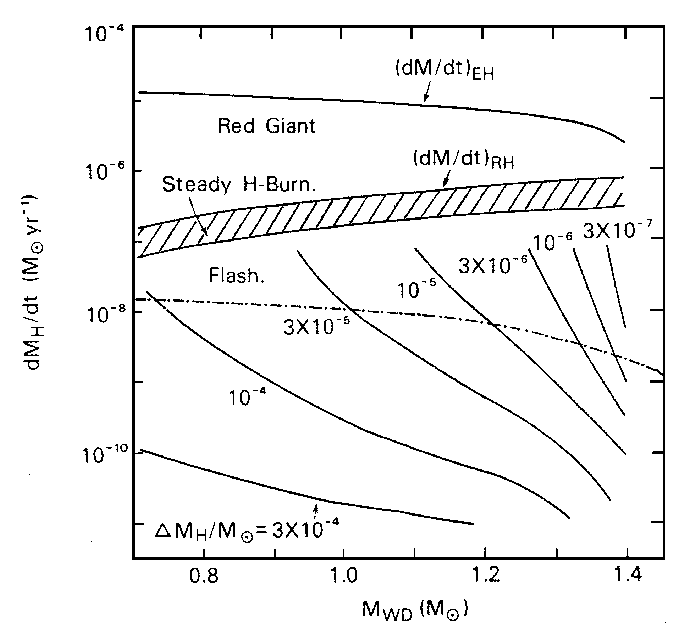
\includegraphics[scale=1.2]{sss-regimes.eps}
        			\caption{Regimes of nuclear burning in surface layers of a white dwarf}
        			\label{fig:regimes-wd}
        		\end{center}
        	\end{figure}
        	
        	These regimes are summarized as follows, for a white dwarf with solar mass:        	
        	\begin{enumerate}
				\item \textbf{Stable hydrogen burning:} For accretion rates within a narrow range of $1-4\times 10^{-7}\,M_{\odot}\,yr^{-1}$, the accreted hydrogen undergoes a stable, continuous burning process on the white dwarf's surface. Crucially, this steady burning occurs without causing significant expansion of the white dwarf itself.
				%For mass accretion rate in the narrow range $1-4\times 10^{-7}\,M_{\odot}\,yr^{-1}$, the accreted hydrogen burns steadily, without any significant radius expansion of the white dwarf.
				\item \textbf{Thermonuclear flashes:} When the accretion rate falls below the threshold for stable burning, the accreted hydrogen ignites in a series of thermonuclear flashes. These explosive events are intermittent, with the frequency of flashes decreasing as the accretion rate diminishes. Concurrently, the individual flashes become more energetic and violent under these conditions.
				%For mass accretion rates below the range of steady burning, the accreted matter burns in flashes, i.e. intermittently. With decreasing accretion rates, the frequency of the flashes decreases and the flashes themselves become more violent.
				\item \textbf{Stable hydrogen burning with radius expansion:} If the accretion rate surpasses the upper limit for stable burning, the white dwarf undergoes dramatic expansion, resembling a red giant star. Despite this expansion, hydrogen burning continues steadily within a thin shell surrounding the white dwarf's core. Intriguingly, this process mirrors the growth of degenerate cores in red giant stars, where hydrogen shell burning is also responsible for the expansion.
				%For mass accretion rates above the range of steady burning, the radius expands to red giant dimensions, and the matter continues to burn steadily within a thin shell around the white dwarf. This, incidentally, corresponds to the growth rate of the degenerate core in red giant stars due to the hydrogen shell burning.
			\end{enumerate}
			
			Hachisu et al. (1996) have calculated that when accretion rates onto a white dwarf significantly exceed the threshold for stable hydrogen burning, a fundamental transformation occurs. Instead of maintaining a static envelope, the accreting matter is expelled in a powerful stellar wind, reaching velocities of approximately 5000 km/s \cite{hachisu96}. Crucially, this high-speed outflow is opaque to soft X-rays, preventing their escape. Consequently, to be observed as a luminous supersoft X-ray source (SSS), the white dwarf must maintain an accretion rate within the stable hydrogen burning regime.
			
			Under these conditions of sustained hydrogen burning, the white dwarf gradually accretes helium while increasing its overall mass. Hachisu et al. suggest that this process can continue until the white dwarf reaches a critical mass of approximately $1.38\,M_{\odot}$, at which point a Type Ia supernova is triggered. This theoretical framework establishes a compelling suggestion of \textit{SSS being the potential progenitors of Type Ia supernovae}.
			%Calculations by Hachisu \emph{et al.} show that when the mass accretion rates are very high, much beyond the steady-burning range, a stellar wind solution replaces the static envelope solution \cite{hachisu96}. This stellar wind flows out from the white dwarfs at high speeds ($\sim 5000$ km/s). Because this stellar wind is opaque to soft X-rays, such radiation do not escape. So long the accretion rate remains within steady-burning range, the white dwarf will be observed as a steady, luminous SSS. According to Hachisu \emph{et al.}, the white dwarf steadily burns hydrogen and accretes helium, thereby increasing its mass up to $1.38\,M_{\odot}$ and then explode as an SN Ia. Therefore, there is a strong suggestion that \emph{SSS could be a possible progenitor for SN Ia}.
		
		\subsection{Possible Companions to a White Dwarf in SSS} \label{introduction:current_status:wd-companions}
			Understanding the nature of the companion star in an SSS system is crucial for elucidating the system's evolutionary history and the mechanisms driving its X-ray emission. This section explores two primary categories of companion stars found in SSS: near main-sequence stars more massive than the white dwarf and symbiotic systems.
		
			\subsubsection{Near main-sequence stars more massive than WDs}
				The simplest configuration for a luminous SSS involves a binary system comprising a white dwarf and a more massive companion star with a radiative envelope, exceeding approximately $1.3\,M_{\odot}$. Once mass transfer from the donor star to the white dwarf commences due to Roche lobe overflow, the binary orbit undergoes shrinkage. The donor star experiences thermal instability, leading to sustained mass transfer until its mass becomes lower than that of the white dwarf, at which point the orbital separation increases \cite{paczynski71}. These systems are termed close-binary supersoft sources (CBSS). Greiner has identified and catalogued\footnote{\url{http://www.mpe.mpg.de/~jcg/sss/ssscat.html}} nine such systems, providing observational support for this model \cite{greiner2000catalog}.
				%The simplest binary configuration that can become a luminous SSS comprises of a white dwarf with a companion star whose mass is larger than about $1.3\,M_{\odot}$ and has a radiative envelope. In such a system, once the donor star overflows its \emph{Roche lobe}, mass transfer to the white dwarf starts, causing its orbit to shrink. The donor becomes thermally unstable and it will continue transferring mass until it becomes less massive of the two and further mass transfer leads to the orbit expansion (Paczynski) \cite{paczynski71}. Such systems are called \emph{close-binary supersoft sources} (CBSS). Nine CBSS have been identified by Greiner \cite{greiner2000catalog,greiner2000catalogOnline}.
				
			\subsubsection{Symbiotic systems}
				Sion et al. (1994) first identified symbiotic systems as another potential host environment for SSS. These systems consist of a white dwarf accreting matter from a red giant companion star. The specific characteristics of the mass transfer process in symbiotic systems can vary depending on the evolutionary stage of the red giant \cite{sion94}. Two primary subtypes of symbiotic SSS are commonly recognized, that provide different modes of mass-transfer.
				%Sion \emph{et al.}\cite{sion94} first showed that a system consisting a red-giant star and a white dwarf is another class of binary systems which can sustain the mass accretion rates necessary for producing supersoft X-rays. Two types of red-giant companions may be expected, providing different modes of mass-transfer.
				
				\begin{enumerate}
					\item One subtype of symbiotic supersoft X-ray sources involves a $1\,M_{\odot}$ red giant companion that is less massive than the white dwarf. These systems typically exhibit orbital periods exceeding 125 days. The red giant component in such systems possesses a degenerate helium core, and its evolutionary processes drive the mass transfer onto the white dwarf. This mass transfer is facilitated by Roche lobe overflow.
					%$1\,M_{\odot}$ red-giant, less massive than the white dwarf. Such a companion overflows its Roche lobe with an orbital period of at least 125 days. The red-giant has a degenerate He core, and its nuclear evolution drives the mass transfer.
					\item Symbiotic systems can also involve a red giant companion in the asymptotic giant branch (AGB) phase of its evolution. Unlike the first subtype, these AGB stars do not fill their Roche lobes. However, they exhibit intense stellar winds, characterized by mass loss rates of the order of $10^{-5}\,M_{\odot}\,yr^{-1}$ and velocities around 30 km/s. A fraction of this ejected material is captured by the white dwarf companion, resulting in accretion rates of about $10^{-7}\,M_{\odot}\,yr^{-1}$. These accretion rates are sufficient to power the white dwarf as a luminous supersoft X-ray source.
					%The red-giant is on the aymptotic giant branch (AGB) and is not filling its Roche lobe, however there is a very strong stellar wind. With mass loss rates from the AGB of the order $10^{-5}\,M_{\odot}\,yr^{-1}$ and stellar wind velocities of around 30 km/s, the aggregate accretion rate can become as large as of the order $10^{-7}\,M_{\odot}\,yr^{-1}$ on a white dwarf, which is sufficient to create a luminous SSS.
				\end{enumerate}
		
		\subsection{Classification Scheme for SSS} \label{introduction:current_status:sss-classification}
			As per di Stefano \emph{et al.} (1996) \cite{distefano96}, binary systems that may appear as luminous SSS may be classified as per table \ref{tab:SSS-class}.
			
			In table \ref{tab:SSS-class}, [A] only those systems are considered in which H-rich material is accreting on the surface of a C-O white dwarf. Here CV = cataclysmic variable, CBSS = close-binary supersoft source and WBSS = wide-binary supersoft source. [B] Two prominent mass transfer mechanisms are mb = magnetic braking and gr = gravitational radiation. [C] $\dot{M}$ is the mass accretion rate on the surface layers of the white dwarf. [D] $P_\text{orb}$ refers to the orbital period of the binary. [D] When $\dot{M}$ is in the correct range (about $\gtrsim 10^{-7}\,M_{\odot}$ yr$^{-1}$), the source burns nuclear fuel more or less steadily (S); for smaller values of $\dot{M}$, hydrogen burns sporadically (R).
			
			\begin{table}[!htb]
				\centering
				\caption{Classification of binary systems that may manifest as SSS}
				\label{tab:SSS-class}
				\begin{tabulary}{\textwidth}{ccccc}
					\hline
					\small{\textbf{[A] System Type}} & \small{\textbf{[B] Mass Transfer Mechanism}} & \small{\textbf{[C] Mass Accretion Rate $\boldsymbol{\dot{M}}$ ($\boldsymbol{M_{\odot}}$ yr$^{-1}$)}} & \small{\textbf{[D] Orbital Period $\boldsymbol{P}_\text{\textbf{orb}}$ (days)}} & \small{\textbf{[E] Steady or Recurrent}}\\
					\hline
					\small{CVs} & \small{mb and/or gr} & \small{$\lesssim 10^{-8}$} & \small{$\lesssim 0.2$} & \small{R}\\
					\hline
					\small{CBSSs} & \small{thermal time scale readjustment of donor} & \small{$\gtrsim 10^{-7}$} & \small{$\sim 0.2-3.0$} & \small{S}\\
					\small{} & \small{} & \small{$\lesssim 10^{-7}$} & \small{$\sim 0.2-\mathscr{O}(10^2)$} & \small{R}\\
					\hline
					\small{WBSSs} & \small{nuclear evolution of donor} & \small{$\gtrsim 10^{-7}$} & \small{$\sim 3.0-\mathscr{O}(10^2)$} & \small{S}\\
					\small{} & \small{} & \small{$\lesssim 10^{-7}$} & \small{$\sim 3.0-\mathscr{O}(10^2)$} & \small{R}\\
					\hline
					\small{Symbiotics (Wind-driven)} & \small{stellar winds from evolved donor} & \small{$\gtrsim 10^{-7}$} & \small{$\mathscr{O}(10^2)$} & \small{S}\\
					\small{} & \small{} & \small{$\lesssim 10^{-7}$} & \small{$\mathscr{O}(10^2)$} & \small{R}\\
					\hline
				\end{tabulary}
			\end{table}
			
		\subsection{Classical Novae} \label{introduction:current_status:CNe}
			Classical novae rank as the third most cataclysmic explosions within a galaxy, surpassed only by supernovae and gamma-ray bursts in terms of energy release. While novae are far less energetic than supernovae, typically liberating luminosities of more than $10^{45}$ erg s$^{-1}$, they occur with significantly higher frequency, making them more commonly observed phenomena within galactic environments.
			%Classical nova explosions are regarded as the third most violent explosions that can occur in a galaxy, preceded by a supernova explosion and a $\gamma$-ray burst. With total liberated energies of more than $10^{45}$ erg s$^{-1}$, novae are less energetic than supernovae, but far more frequent within a galaxy.
			
			The prevailing model for classical novae, as outlined by Krautter (2008), posits their occurrence within cataclysmic binary systems. These systems comprise a white dwarf primary accreting matter from a main-sequence or slightly evolved companion star. The mass transfer process, facilitated by Roche lobe overflow, channels material towards the white dwarf through the inner Lagrangian point, forming an accretion disk.
			
			The conditions leading to a thermonuclear runaway on the white dwarf's surface are intricately linked to factors such as the white dwarf's mass and luminosity, the accretion rate, and the chemical composition of the accreted material \cite{starrfield89}. As hydrogen-rich matter accumulates, it undergoes compression and heating. When temperatures within the accreted layer surpass $10^8$ K, runaway thermonuclear fusion ignites, releasing vast amounts of energy. The peak luminosity during these events can approach the Eddington limit $L_\text{Edd}$, a critical threshold beyond which radiation pressure exceeds gravitational force, imposing an upper limit on the luminosity of a star.
			%As per the accepted standard model described by Krautter, nova explosions occur in cataclysmic binary systems \cite{krautter08}. In such systems, one member is a white dwarf and the other member is a main-sequence or slightly evolved star that fills its Roche lobe, with mass transfer from the secondary to the white dwarf taking place through the inner Lagrangian point, leading to the formation of an accretion disk. The evolution of a thermonuclear runaway on the white dwarf depends upon the mass and luminosity of the white dwarf, the mass accretion rate, and the chemical composition of the accreted layer \cite{starrfield89}. The temperature in the H-burning zone can grow to values exceeding $10^8$ K, while luminosities are of the order of the Eddington luminosity $L_\text{Edd}$ (\textit{Eddington luminosity}, or \textit{Eddington limit}, is the maximum luminosity a body can achieve under the state of \textit{hydrostatic equilibrium}).
			
			X-ray observations have emerged as a pivotal tool for investigating the high-temperature phases associated with nova outbursts.
 While these observations have yielded valuable insights, the relatively small number of novae studied in the X-ray band compared to other spectral domains (optical, infrared, ultraviolet) has hindered the development of a comprehensive understanding of novae in this energy range. Nevertheless, two primary mechanisms have been proposed to explain X-ray emission from novae.
			%X-ray astronomy has turned out to be a powerful tool for the study of novae outburst, since the X-ray regime is best suited to study such hot phases. X-ray observations have provided many fundamental and in part unexpected results. However, so far the picture that emerged from X-ray observations of novae is far less systematic than the one from other spectral regimes, since unlike in the optical, infrared, or ultraviolet regime, only few objects were observed in X-rays.
			
			%Two viable mechanisms for X-ray emission from a nova outburst are described in brief here.
			
			\subsubsection{Thermal radiation from hot white dwarf}
				Following a nova eruption, the energy released from thermonuclear burning is rapidly transported to the white dwarf's surface. This influx of energy dramatically increases the star's effective temperature. For a white dwarf radiating at its Eddington luminosity $L_\text{Edd}$, the temperature could be expected to be several thousand kelvins, depending on the white dwarf's mass. Consequently, the nova enters a phase of intense soft X-ray emission, characterized by a spectral energy distribution (SED) resembling that of a hot stellar atmosphere.
				
				As the nova ejecta expand outward, they form a cooling pseudo-photosphere. This expansion leads to a rapid decrease in temperature and a corresponding decline in X-ray flux due to the increasing opacity of the expanding envelope to X-rays \cite{krautter96}.
				%After the energy created by nuclear reactions has reached the surface of the white dwarf, the effective surface temperature increases rapidly.For luminosity of the order of $L_\text{Edd}$ and unit white dwarf radius, the temperature could be expected to be several thousand kelvins (depending on the white dwarf mass). The nova then emits strong soft X-rays with the \emph{spectral energy distribution} (SED) of a hot stellar atmosphere. After the ejection of the nova shell, the temperature of the expanding pseudo-photosphere decreases rapidly with increasing radius. Also, the X-ray flus drops since the expanding envelope becomes opaque to X-rays (Krautter \emph{et al.}) \cite{krautter96}.
				
			\subsubsection{X-ray emission from circumstellar material}
				A second mechanism contributing to X-ray emission in nova systems involves interactions between the expanding nova ejecta and the surrounding circumstellar environment. This interaction can occur either within the ejected material itself or between the ejecta and pre-existing circumstellar matter. As proposed by Balman et al. (1998), shock waves generated by these collisions can reach temperatures of several keV, producing thermal \textit{bremsstrahlung} radiation in the X-ray band \cite{balman98}.
				%In the circumstellar material surrounding the nova system, the expanding nova shell and/or a nova wind interact with pre-existing material of with each other. In this mechanism, as per Balman \emph{et al.} \cite{balman98}, strong shocks giving rise to a thermal \emph{bremsstrahlung} SED with temperatures up to several keV may be expected.

    \section{Statement of the Research Problem} \label{introduction:problem_statement}
    	To understand the nature of binary systems emitting supersoft X-rays by the analysis of their spectra and the study of their variabilities in X-ray and visible/ultraviolet regimes.
        
    \section{Hypothesis} \label{introduction:hypothesis}
    	The radiative processes governing supersoft X-ray sources are much complex than previously assumed and could include non-steady states, NLTE and stellar winds.
    
    \section{Objectives of the Study} \label{introduction:objectives}
    	\begin{enumerate}
    		\item To develop a robust and consistent model that accurately fits the continuum spectra of supersoft X-ray sources (SSS) across different sources, and using multi-observatory science data.
    		
    		\item To demonstrate that the spectra of SSS within the 0.2--1.0 keV photon energy range can be satisfactorily modeled using Non-Local Thermodynamic Equilibrium (NLTE) components, and to validate this approach across multiple sources.
    		
    		\item To investigate and distinguish the absorption components due to the source atmosphere and the interstellar medium (ISM) in the spectra of SSS from both the Milky Way and the Large Magellanic Cloud (LMC).
    		
    		\item To compute stellar parameters for the selected SSS using the best-fit models, thereby constraining their luminosities, effective temperature and column densities.
    		
    		\item To investigate and distinguish the absorption components due to the source atmosphere and the interstellar medium (ISM) in the spectra of SSS from both the Milky Way and the Large Magellanic Cloud (LMC).
    		
    		\item To identify and analyze the differences in spectral characteristics, such as absorption edges, between SSS in the Milky Way and those in the LMC, and to understand the underlying reasons for these differences.
    		
    		\item To develop a software tool that accesses publicly available atomic data and overlays the relevant atomic lines on the grating spectra of SSS, thereby facilitating preliminary line identification for astronomers.
    		
    		\item To study a grid of models for fitting the grating spectra of SSS, comparing their fitting statistics.
    	\end{enumerate}
%    	\begin{enumerate}
%			\item To study different models for spectral fitting of the list of sources.
%			\item To study the temporal variability of the list of sources.
%			\item To propose and calculate novel stellar atmospheric models and generate the associated synthetic spectra.
%			\item To develop corresponding software models that can be used in XSPEC.
%			\item To compute stellar parameters for the list of sources using the best-fit models.
%			\item To propose models for the interstellar medium by studying the absorption edges in the observed spectra of the identified sources.
%		\end{enumerate}
    
    \section{Significance of the Study} \label{introduction:significance}
    	The study of SSS is crucial for understanding the physics and evolution of compact binary systems, such as white dwarfs and their interactions with companion stars. This research addresses several key challenges in modeling the spectra of SSS, providing significant advancements in the field of high-energy astrophysics.
    	
    	Firstly, developing a robust and consistent model that accurately fits the continuum spectra of SSS across different sources and using multi-observatory data is fundamental to obtaining reliable measurements of their physical parameters. This helps in better understanding the nature of these sources, their life-cycle, and their role in the broader context of stellar evolution.
    	
    	Secondly, demonstrating that the spectra of SSS within the 0.2--1.0 keV photon energy range can be satisfactorily modelled using Non-Local Thermodynamic Equilibrium (NLTE) components fills a crucial gap in current astrophysical models. NLTE modeling provides a more accurate representation of the physical conditions in the atmospheres of SSS, leading to more precise determinations of their effective temperatures, luminosities, and column densities. Additionally, the spectra fitted within this range can be extrapolated to lower energies (or higher wavelengths) and compared with observations made in the UV/optical regime. This cross-validation enhances the reliability of the models and provides a comprehensive understanding of the sources across different wavelengths.
    	
    	Thirdly, investigating the absorption components due to the source atmosphere and the interstellar medium (ISM) in the spectra of SSS from both the Milky Way and the Large Magellanic Cloud (LMC) adds another layer of understanding regarding the interaction of X-ray photons with intervening matter. This not only enhances our comprehension of the local environments of these sources but also provides insights into the composition and distribution of the ISM in different galactic environments.
    	
    	Additionally, by computing stellar parameters using best-fit models, the study places constraints on the luminosities, effective temperatures, and column densities of SSS, contributing valuable data to the field of stellar astrophysics. Identifying and analyzing differences in spectral characteristics, such as absorption edges, between SSS in the Milky Way and those in the LMC, sheds light on the unique astrophysical processes at play in different galactic contexts.
    	
    	Furthermore, the development of a software tool for preliminary line identification using publicly available atomic data is a significant contribution to the astronomical community. This tool facilitates the identification of key atomic lines in grating spectra, enabling more detailed and accurate spectral analysis.
    	
    	Finally, by studying a grid of models for fitting the grating spectra of SSS and comparing their fitting statistics provides a comprehensive evaluation of different modeling approaches, ensuring the selection of the most appropriate models for accurate spectral fitting.
%        Different observations of SSS, separated from each other by months, exhibit new SSS and, more importantly, only a few members which are common to previous observations. This clearly implies that such sources have ``on/off'' phases that take place over time intervals spanning months. It is indeed certain that, with continuous monitoring of SSS over time-frames in decades, the number of SSS discovered would increase dramatically.
%        
%        Study of the X-ray variability of SSS is expected to provide valuable clues to the dynamics of the SSS -- not only for those already well-studied, but also for newly-discovered sources for which satisfactory models are yet to be arrived at. Simultaneously, the study of the features present in their spectra, using robust models, promises to shed light on the physics behind the processes taking place in SSS. In addition, a careful study of the absorption edges, due to various metals, exhibited in their high-resolution spectra can provide clues to the structure and composition of the intervening interstellar medium.
%        
%        Our present understanding of nuclear-burning white dwarfs and progenitors of type Ia supernovae explosions can evolve significantly with further monitoring and study of SSS. The reason for this being the fact that these are observed to be accompanied by a phase of supersoft X-ray emission.
    
    \section{Contribution of the Thesis} \label{introduction:thesis_contribution}
    	The current thesis makes several important contributions to the field of high-energy astrophysics, particularly in the study of supersoft X-ray sources:
    	\begin{enumerate}[I.]
    		\item \textbf{Development of a Robust Spectral Model:} The current thesis presents a robust and consistent model that accurately fits the continuum spectra of SSS across different sources using data from multiple observatories. This model provides a reliable framework for analyzing and interpreting SSS spectra.
    		
    		\item \textbf{Validation of NLTE Modeling:} By demonstrating that the spectra of SSS within the 0.2--1.0 keV photon energy range can be satisfactorily modeled using NLTE components, this research validates a crucial approach for studying the physical conditions in the atmospheres of these sources. This contributes to more accurate determinations of their temperatures and luminosities. Moreover, the extrapolation of these models to UV/optical observations strengthen the consistency and reliability of the models.
    		
    		\item \textbf{Analysis of Absorption Components:} The investigation into the absorption components due to the source atmosphere and the ISM in the spectra of SSS from both the Milky Way and the LMC provides a deeper understanding of the interactions between X-ray photons and intervening matter. This analysis enhances our knowledge of the local environments of SSS and the ISM's composition in different galaxies.
    		
    		\item \textbf{Computation of Stellar Parameters:} The thesis provides precise computations of stellar parameters for the selected SSS, including luminosities, effective temperatures, and column densities. These results are valuable for constraining models of these sources and understanding their physical properties.
    		
    		\item \textbf{Identification of Spectral Absorption Edges:} By identifying and analyzing differences in absorption edges, between SSS in the Milky Way and those in the LMC, the research offers insights into the unique astrophysical processes in different galactic environments. This helps explain the variations in the observed spectra of SSS.
    		
    		\item \textbf{Development of a Line Identification Tool:} The development of a Python-based software tool\footnote{\url{https://github.com/pararover/xmmrgs_lines}} that accesses atomic data and overlays relevant atomic lines on the grating spectra of SSS is a practical contribution. This tool aids astronomers in performing preliminary line identification, facilitating further spectral analysis and interpretation.
    		
    		\item \textbf{Evaluation of Spectral Models:} By studying a grid of models for fitting the grating spectra of SSS and comparing their fitting statistics, the thesis provides a comprehensive evaluation of different modeling approaches. This ensures the selection of the most suitable models for accurate spectral fitting, enhancing the reliability of spectral analysis.
    	\end{enumerate}
        %The present study obtains an unprecedented model fit of the complex high-resolution spectrum of the source named \mrvel\ with the RGS instrument of the XMM-Newton observatory. In the process, we propose a hypothesis for the physical processes that govern the radiation from this particular X-ray binary. We also apply a similar spectral study on other supersoft X-ray sources with similar spectral characteristics.
    
    %\section{Organization of the Thesis} \label{introduction:thesis_organization}
    %    \lipsum[10]
